\documentclass[xcolor=dvipsnames]{beamer}
\usepackage{beamerthemelined}
\usepackage{pstricks}
\usepackage{animate}

\setbeamertemplate{navigation symbols}{}
\usepackage{caption}
\captionsetup{textfont={small,bf,color=cyan}}
\captionsetup{labelformat=empty}

\usepackage{ifthen,xifthen}
\newenvironment{items}[1][]
{\begin{itemize}
    \ifthenelse{\isempty{#1}}
    {\setlength{\itemsep}{12pt}}{\setlength{\itemsep}{#1}}}
  {\end{itemize}}

%%% Standard math:
\usepackage{amsfonts,amssymb,amsmath,amsthm} % Math packages
\usepackage{braket} % Bra-ket notation stuff
\newcommand{\st}{\displaystyle} % For making small math big
\renewcommand{\t}{\text} % For text in math environment
\renewcommand{\c}{\cdot} % Multiplication dot in math
\newcommand{\f}[2]{\dfrac{#1}{#2}} % Shortcut for fractions
\newcommand{\p}[1]{\left(#1\right)} % Parenthesis
\renewcommand{\sp}[1]{\left[#1\right]} % Square parenthesis
\renewcommand{\set}[1]{\left\{#1\right\}} % Curly parenthesis
\newcommand{\abs}[1]{\left|#1\right|} % Absolute value

%%% Physics symbols, vectors
\renewcommand{\epsilon}{\varepsilon} % Prettier epsilon
\renewcommand{\phi}{\varphi} % Prettier phi
\renewcommand{\l}{\ell} % Prettier l
\renewcommand{\v}[1]{\boldsymbol{\mathrm{#1}}} % Bold vectors
\newcommand{\uv}[1]{\hat{\boldsymbol{\mathrm{#1}}}} % Unit vectors
\newcommand{\del}{\v\nabla} % Del operator
\renewcommand{\d}{\partial} % Partial d
\newcommand{\fd}[2]{\f{d #1}{d #2}} % Derivative
\newcommand{\sd}[2]{\f{d^2 #1}{d^2 #2}} % Derivative
\newcommand{\fpd}[2]{\f{\d #1}{\d #2}} % Partial derivative
\newcommand{\spd}[2]{\f{\d^2 #1}{\d^2 #2}} % Partial derivative

\title{Investigating an Optical Vortex (THIS BEGS FOR A NEW TITLE!!!111!!!@!@!!!!)}
\author{Aaron Kratzer, David Grant, Paho Lurie-Gregg,
  Michael Perlin, Grant Sherer}
\date{06 December 2013}

\begin{document}

\begin{frame}
  \maketitle
\end{frame}

\begin{frame}
	\frametitle{Generation - Multilayer Spiral Phase Plate}
  \begin{columns}[c]
    \column{2.5in}
    \begin{items}
    \item SiO$_2$ is deposited onto a substrate using an electron beam
    \item Since the plate thickness varies with $\phi$, the phase
      develops the $\phi$ dependence that produces a helical wave
      front
    \end{items}
    \column{2in}
    \begin{figure}
      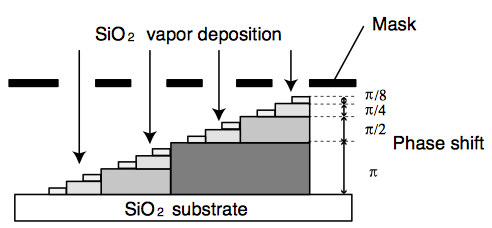
\includegraphics[width=\columnwidth]{MSPP.jpg}
      \caption{SiO$_2$ Phase Plate}
      \label{MSPP}
    \end{figure}
  \end{columns}
\end{frame}

\begin{frame}
	\frametitle{Generation - Computer Generated Holography}
  \begin{items}
  \item A reference wave and a particular object wave are combined to
    form an interference pattern.
  \item The interference pattern is then produced as a hologram
    filament.
  \item When a beam propagates through this filament, the first order
    diffraction beam contains the optical vortex.
  \end{items}
\end{frame}

\begin{frame}
  \centering
    \begin{align*}
  \v A\p{r,\phi,z}&=A_0\f{w_0}{w}\sp{\f{r\sqrt 2}{w}}^\ell
  L^{\p{\ell}}_p\sp{2\f{r^2}{w^2}}\exp\sp{-\f{r^2}{w^2}}
  \exp\sp{-i\f{kr^2z}{2\p{z^2+z_R^2}}} \\
  &~~~~\times\exp\sp{i\p{2p+\ell+1}\arctan\p{\f z{z_R}}}
  \exp\p{i\ell\phi}\exp\p{-i\omega t} \uv x\\
   w&=w_0\sqrt{1+z^2/z_R^2}\\
    L^{\p{\ell}}_p\p{x}
 & =\sum_{m=0}^p\p{-1}^m\f{\p{p+\ell}!}{\p{p-m}!\p{\ell+m}!m!}x^m\\
  z_R&=\f12 kw_0^2
\end{align*}
 \end{frame}

\begin{frame}
\begin{align*}
  L^{\p{3}}_1\p{x}=-x+4\\
  \v E=i\omega\v A &&& \v B=-\del \times\v A
\end{align*}
\end{frame}

\begin{frame}
\begin{align*}
 u&=\f12\p{\epsilon E^2+B^2/\mu} \\
  \v S&=\v E\times\v B/\mu \\
    I&=\f{c\epsilon}2E^2=\f c2\epsilon\omega^2A_I^2=cu/2\\
\end{align*}
\end{frame}

\begin{frame}
\begin{align*}
 \sigma_{ij}&=\epsilon\p{E_iE_j-\f12\delta_{ij}E^2}
  +\f1\mu\p{B_iB_j-\f12\delta_{ij}B^2} \\
    &=\delta_{ij}\f12\p{\epsilon
    E^2+B^2/\mu}=\delta_{ij}u\\
 f_i&=\d_k\sigma_{ik}-\d_tS_i/c^2=\d_iu-\delta_{iz}\d_tu/c
\end{align*}
\end{frame}

% \begin{frame}
%  \begin{figure}[h]
%    \centering
%    \animategraphics[width=.9\columnwidth, loop]{5}{anim/slice-Ex-}{01}{14}
%  \end{figure}
% \end{frame}

% \begin{frame}
%  \begin{figure}[h]
%    \centering
%    \animategraphics[width=.9\columnwidth, loop]{5}{anim/slice-By-}{01}{14}
%  \end{figure}
% \end{frame}

% \begin{frame}
%  \begin{figure}[h]
%    \centering
%    \animategraphics[width=.9\columnwidth, loop]{5}{anim/slice-Bz-}{01}{14}
%  \end{figure}
% \end{frame}

% \begin{frame}
%  \begin{figure}[h]
%    \centering
%    \animategraphics[width=.9\columnwidth, loop]{5}{anim/slice-Sy-}{01}{14}
%  \end{figure}
% \end{frame}

% \begin{frame}
%  \begin{figure}[h]
%    \centering
%    \animategraphics[width=.9\columnwidth, loop]{5}{anim/slice-Sz-}{01}{14}
%  \end{figure}
% \end{frame}

%---begining of presentation---




%-----Aaron's Application stuff--------
\begin{frame}
	\frametitle{Optical Vortex Application: Twisted Radio Waves}
	\begin{center}
		\emph{Encoding many channels in the same frequency through radio vorticity: first experimental test.}
	\end{center}
	\begin{minipage}{0.49\textwidth}
	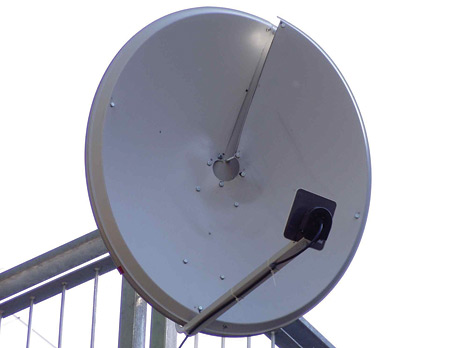
\includegraphics[width=\textwidth]{helical_dish}
	\end{minipage}
	\begin{minipage}{0.49\textwidth}
		\begin{items}
		\item Multiple signals transmitted on the same frequency.
		\end{items}
	\end{minipage}

\end{frame}

\end{document}
